\chapter{Experiments}
\label{experiments}

The experiments in this work were made to test whether the REFINED model can work better than other state-of-the-art methods. The first experiment tested the whole technique in a situation similar to real-life problems. The hope was that the model would show results above the other methods, such as RFC or Dense Neural Networks, commonly used in classification problems. The second experiment is designed to test the hypothesis that using the images transformed by the REFINED core as the input into a CNN increases the performance of its prediction capabilities.

\section{Experiment 1: Overall comparison}
\label{first_experiment}

The first experiment consists of comparing all the methods as a whole. Firstly, I run hyperparameter optimization for each method as described in its description. Then, with these hyperparameters, a model is trained. The \textit{chen11} dataset is used for training, and metrics are calculated on the \textit{coach420} dataset. With this experiment, I want to test whether REFINED performs better on this dataset than other state-of-the-art approaches, such as Random Forest Classifier or Dense Neural Network.

For this experiment, I took the training dataset and split it into 5 parts. Then, for each model architecture, 5 models were trained, each on $\frac{4}{5}$ of the training dataset. First, I calculated the AUC for each model. Then, I optimize the best threshold based on the F1 score. This threshold was then used for all remaining metrics. The mean ($\mu$) and the standard deviation ($\sigma$) were then calculated for each metric. 
   
\begin{figure}
    \centering
    \includegraphics[width=0.75\linewidth]{auc.png}
    \caption{AUC for each model. Confidence intervals have the size of the standard deviation of the model's 5 results. $\mu$ and $\sigma$ were calculated from 5 runs on different dataset splits.}
    \label{fig:auc}
\end{figure}

\begin{figure}
    \centering
    \includegraphics[width=0.75\linewidth]{metric_comparisons.png}
    \caption{F1 score, Precision, Recall, and Accuracy for each model. Thresholds were chosen for the best possible F1 score. The plot has been created the same way as figure ~\ref{fig:auc}}.
    \label{fig:f1_et_al}
\end{figure}

\begin{figure}%
\centering
\begin{subfigure}{0.45\textwidth}
    \centering
    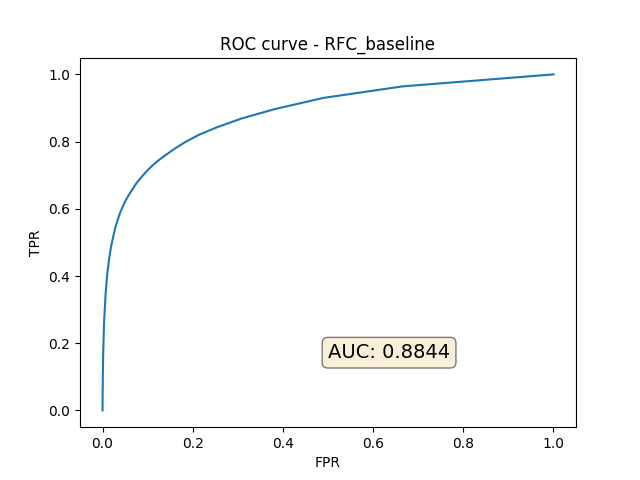
\includegraphics[width=0.95\linewidth]{roc_baseline.png}
    \caption{P2Rank RFC}
\end{subfigure}%
\begin{subfigure}{0.45\textwidth}
    \centering
    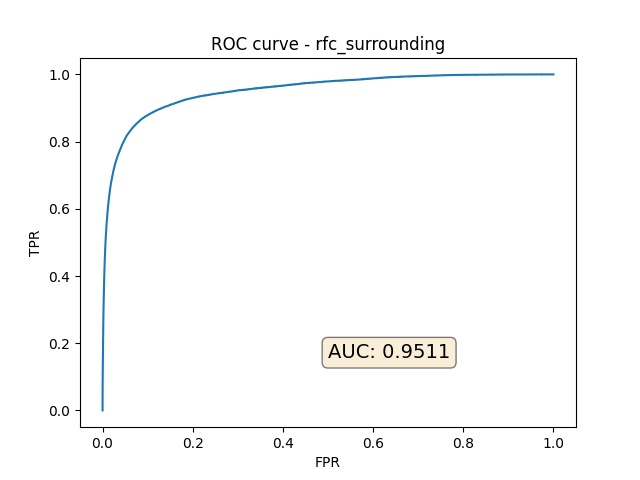
\includegraphics[width=0.95\linewidth]{roc_big_rfc.png}
    \caption{RFC Surrounding}
\end{subfigure}
\begin{subfigure}{0.45\textwidth}
    \centering
    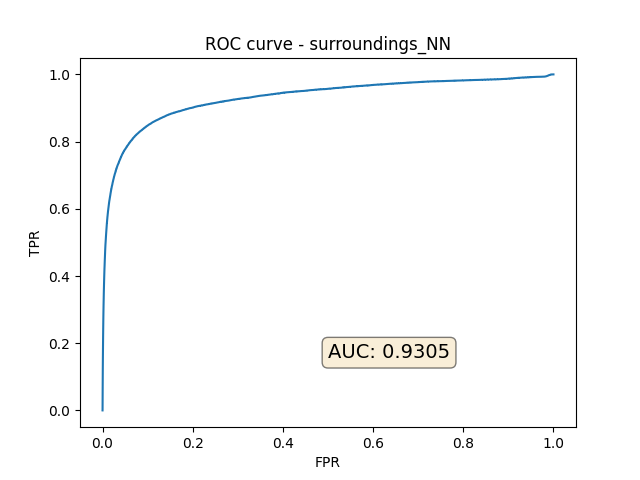
\includegraphics[width=0.95\linewidth]{roc_nn.png}
    \caption{NN}
\end{subfigure}%
\begin{subfigure}{0.45\textwidth}
    \centering
    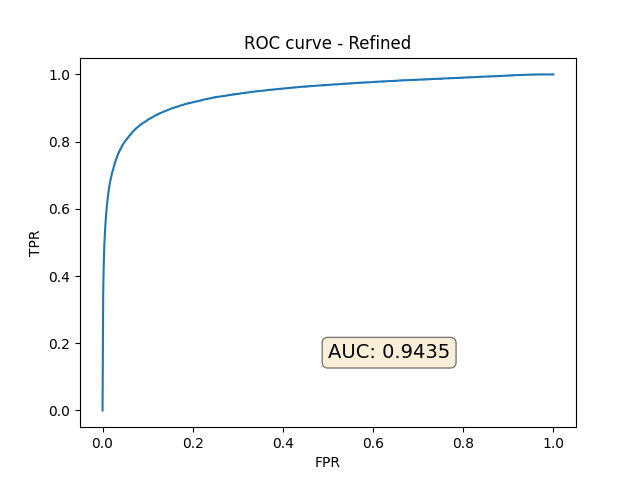
\includegraphics[width=0.95\linewidth]{refined_roc.png}
    \caption{REFINED model}
\end{subfigure}
\begin{subfigure}{0.45\textwidth}
    \centering
    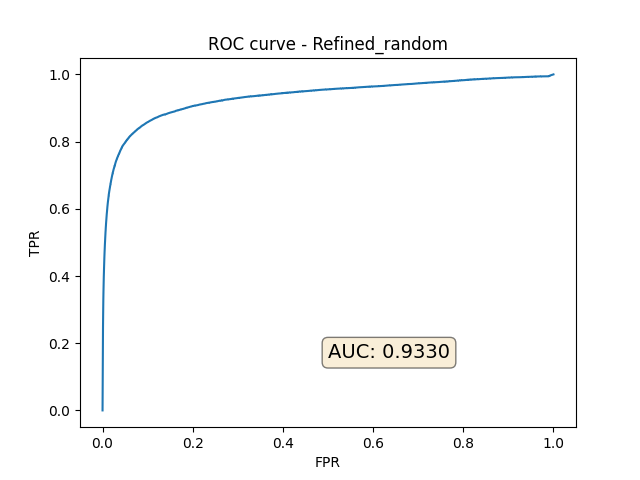
\includegraphics[width=0.95\linewidth]{random_roc.png}
    \caption{Random CNN}
\end{subfigure}%
\begin{subfigure}{0.45\textwidth}
    \centering
    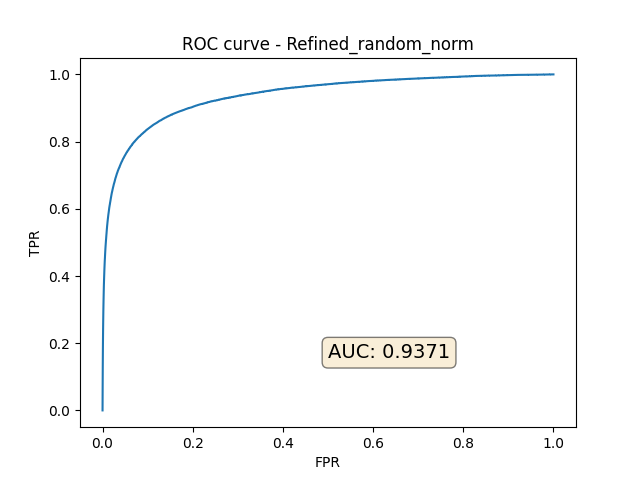
\includegraphics[width=0.95\linewidth]{norm_roc.png}
    \caption{Normalized CNN}
\end{subfigure}%
\caption{ROC curves of the instances with the highest AUC of each individual model type from the first experiment.}
\label{fig:roc_curves}
\end{figure}

\begin{figure}
    \centering
    \includegraphics[width=0.75\linewidth]{ab1.png}
    \caption{One-way student t-test testing whether model on the y-axis has a higher mean AUC compared to the model on the x-axis. Blacked-out squares represent p-values $> 0.01$. For better understandability, the $-log_{10}(p_value)$ is shown.}
    \label{fig:ab1}
\end{figure}

The AUC scores for each model are shown in ~\ref{fig:auc}. In ~\ref{fig:ab1} are shown the results of running the Student's t-test to test whether the means of AUC are different from each other. As can be seen from the first graph, there are no significant differences between models using the surroundings dataset as input except for \textit{RFC Surrounding} model slightly outperforming most other models. But, even though these tests show positive results, the differences are very small and probably just dataset dependant.

\subsection{Found hyperparameters}

Before the models were trained, I ran hyperparameter optimization on them. The resulting architectures then are as follows:
\begin{itemize}
    \item \textbf{RFC Surrounding}:
    \begin{itemize}
        \item n-estimators=500
        \item min-samples-split=5
        \item max-features=sqrt
        \item max-depth=10
    \end{itemize}
    \item \textbf{NN} \textit{(lr=5e-4)} 36k parameters:
    \begin{itemize}
        \item InputLayer(1140)
        \item Dense(32, activation=ReLU)
        \item Dense(1, activation=sigmoid)
    \end{itemize}
    \item \textbf{REFINED} \textit{(lr=5e-4)} 1.8M parameters:
    \begin{itemize}
        \item InputLayer((38, 30))
        \item Conv2D(filters=1024, stride=3, kernel-size=5, activation=ReLU)
        \item Flatten()
        \item Dense(16, activation=ReLU)
        \item Dense(1, activation=sigmoid)
    \end{itemize}
    \item \textbf{Random CNN} \textit{(lr=5e-5)} 1.0M parameters:
    \begin{itemize}
        \item InputLayer((38, 30))
        \item Conv2D(filters=128, stride=2, kernel-size=3, activation=ReLU)
        \item Flatten()
        \item Dense(32, activation=ReLU)
        \item Dense(1, activation=sigmoid)
    \end{itemize}
    \item \textbf{Normalized CNN} \textit{(lr=5e-5)} 25M parameters:
    \begin{itemize}
        \item InputLayer((38, 30))
        \item Conv2D(filters=128, stride=1, kernel-size=3, activation=ReLU)
        \item Conv2D(filters=179, stride=1, kernel-size=3, activation=ReLU)
        \item Conv2D(filters=250, stride=1, kernel-size=3, activation=ReLU)
        \item Flatten()
        \item Dense(128, activation=ReLU)
        \item Dense(1, activation=sigmoid)
    \end{itemize}
\end{itemize}

\subsection{A bit more into CNN training}

All three CNNs in this experiment have very different hyperparameters. 

\begin{figure}%
\centering
\begin{subfigure}{0.45\textwidth}
    \centering
    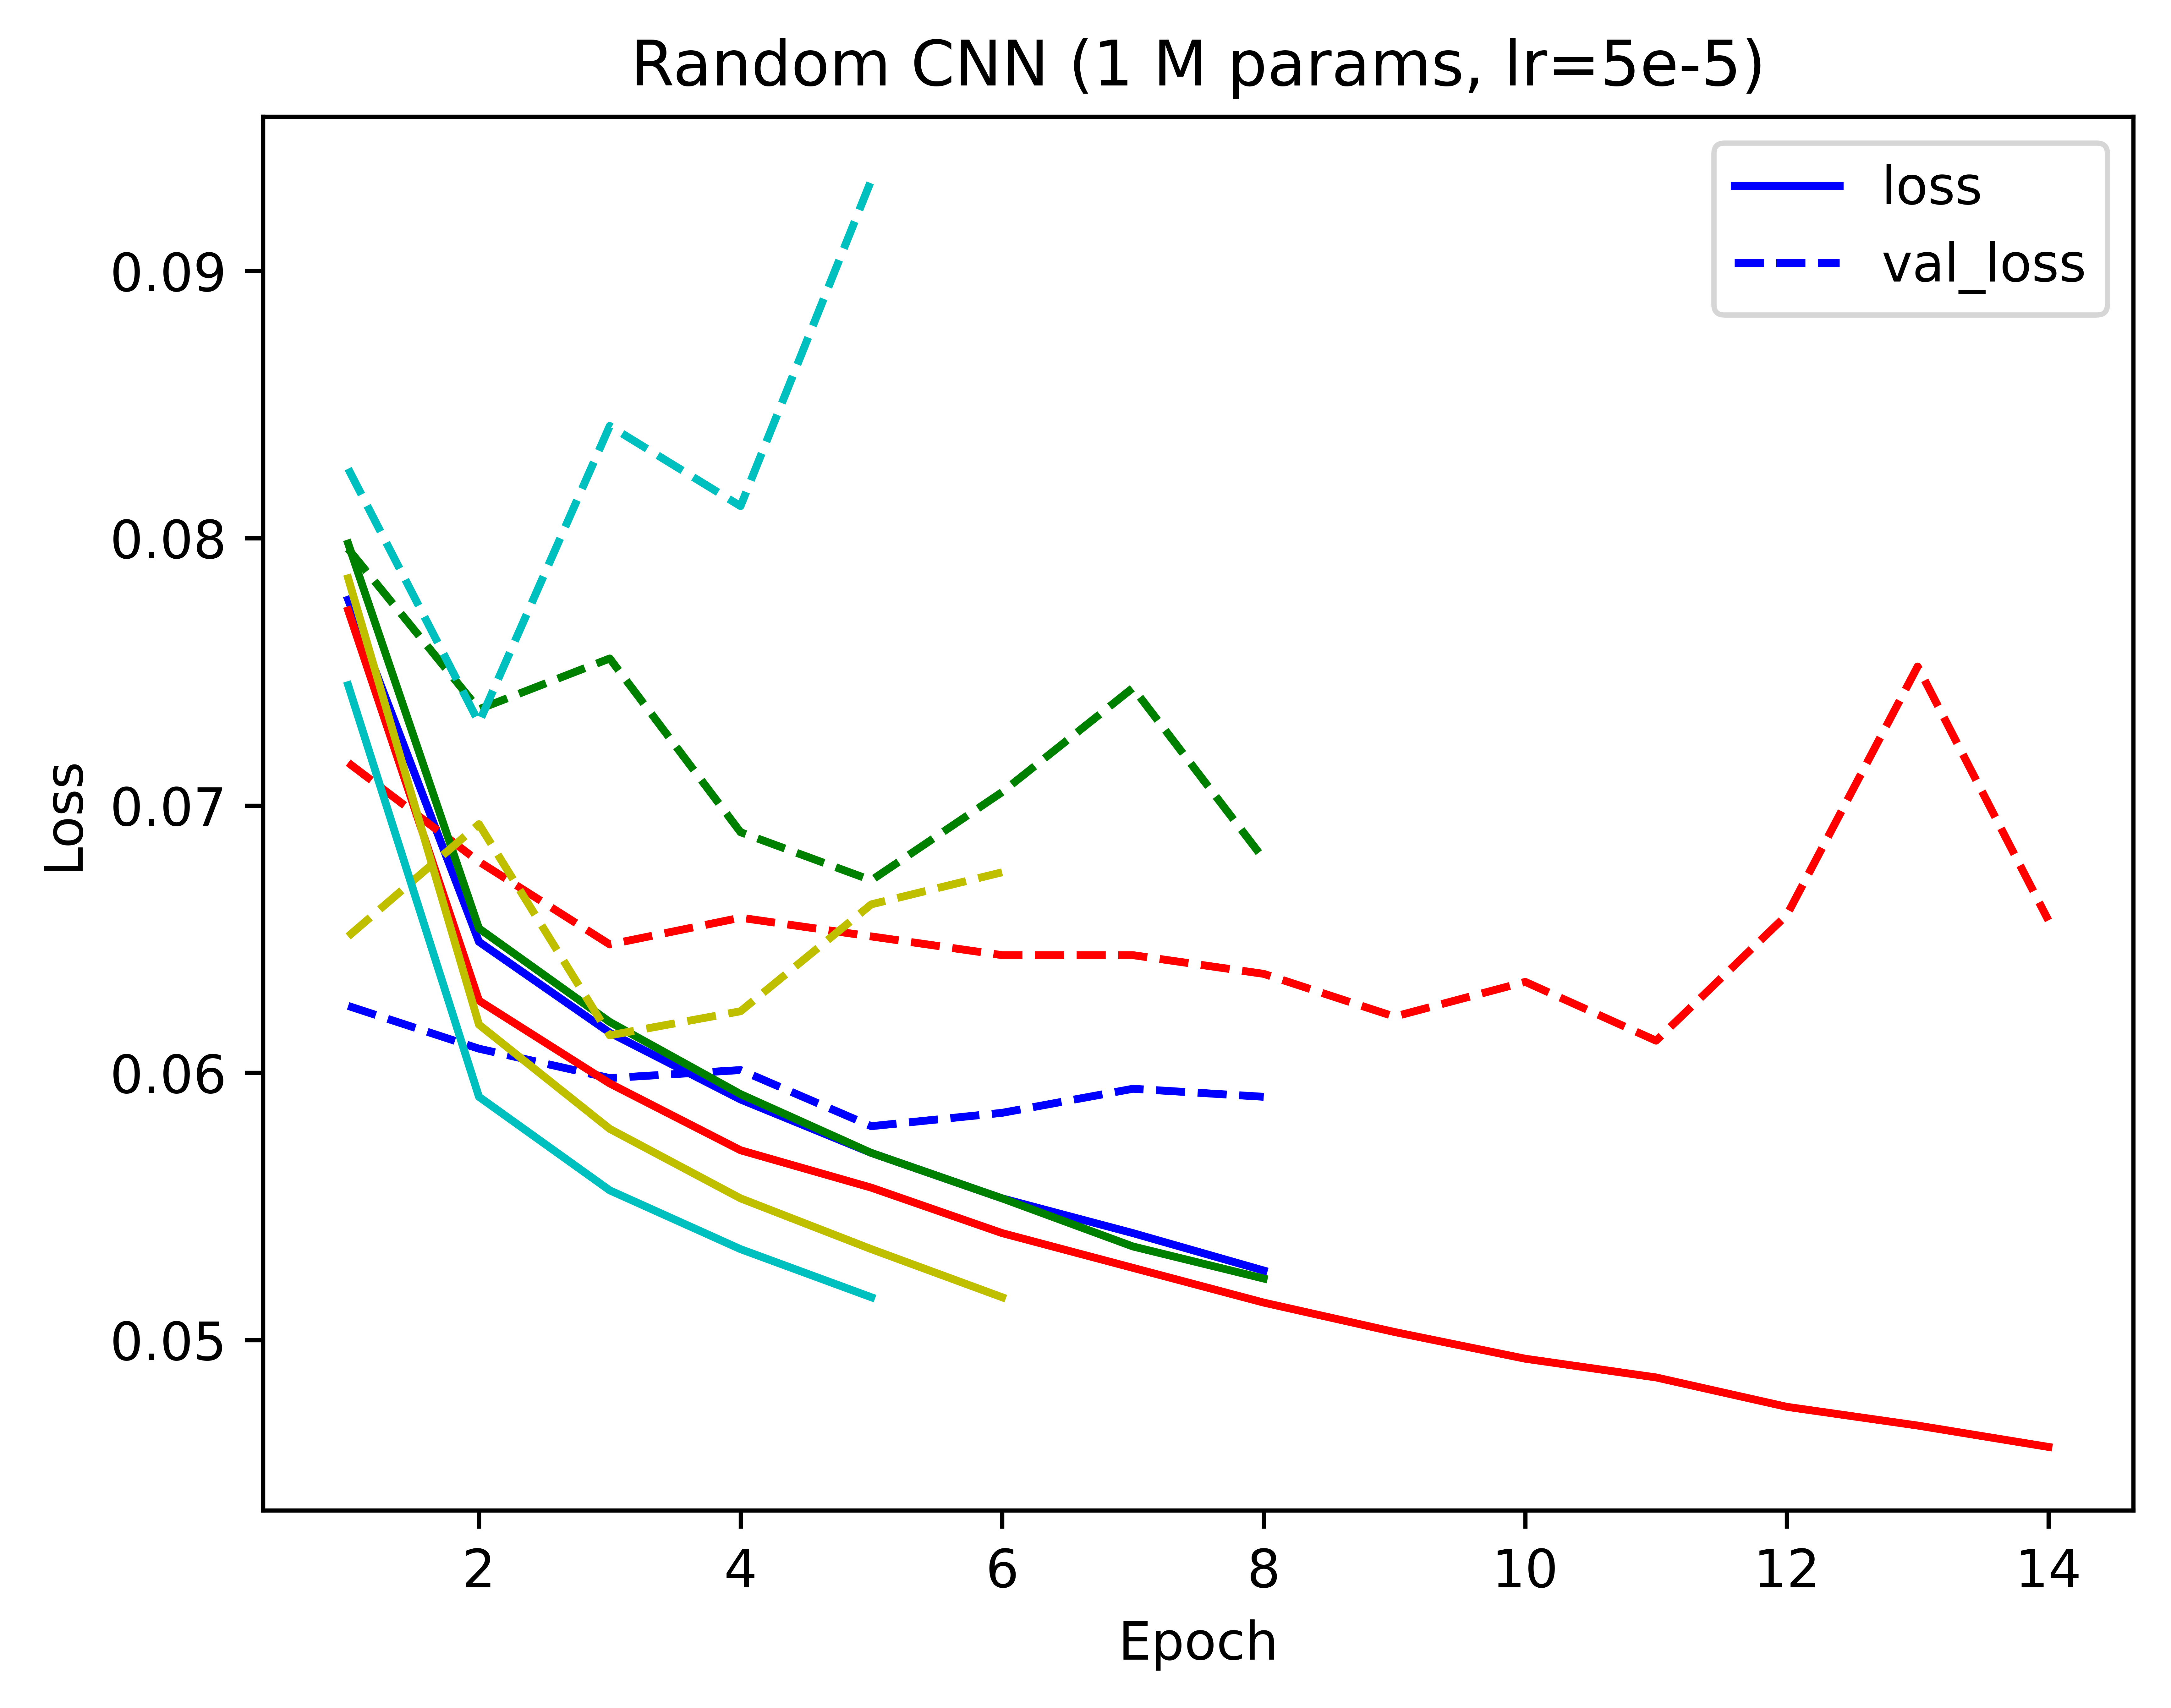
\includegraphics[width=1\linewidth]{Random CNN_loss.png}
\end{subfigure}%
\begin{subfigure}{0.45\textwidth}
    \centering
    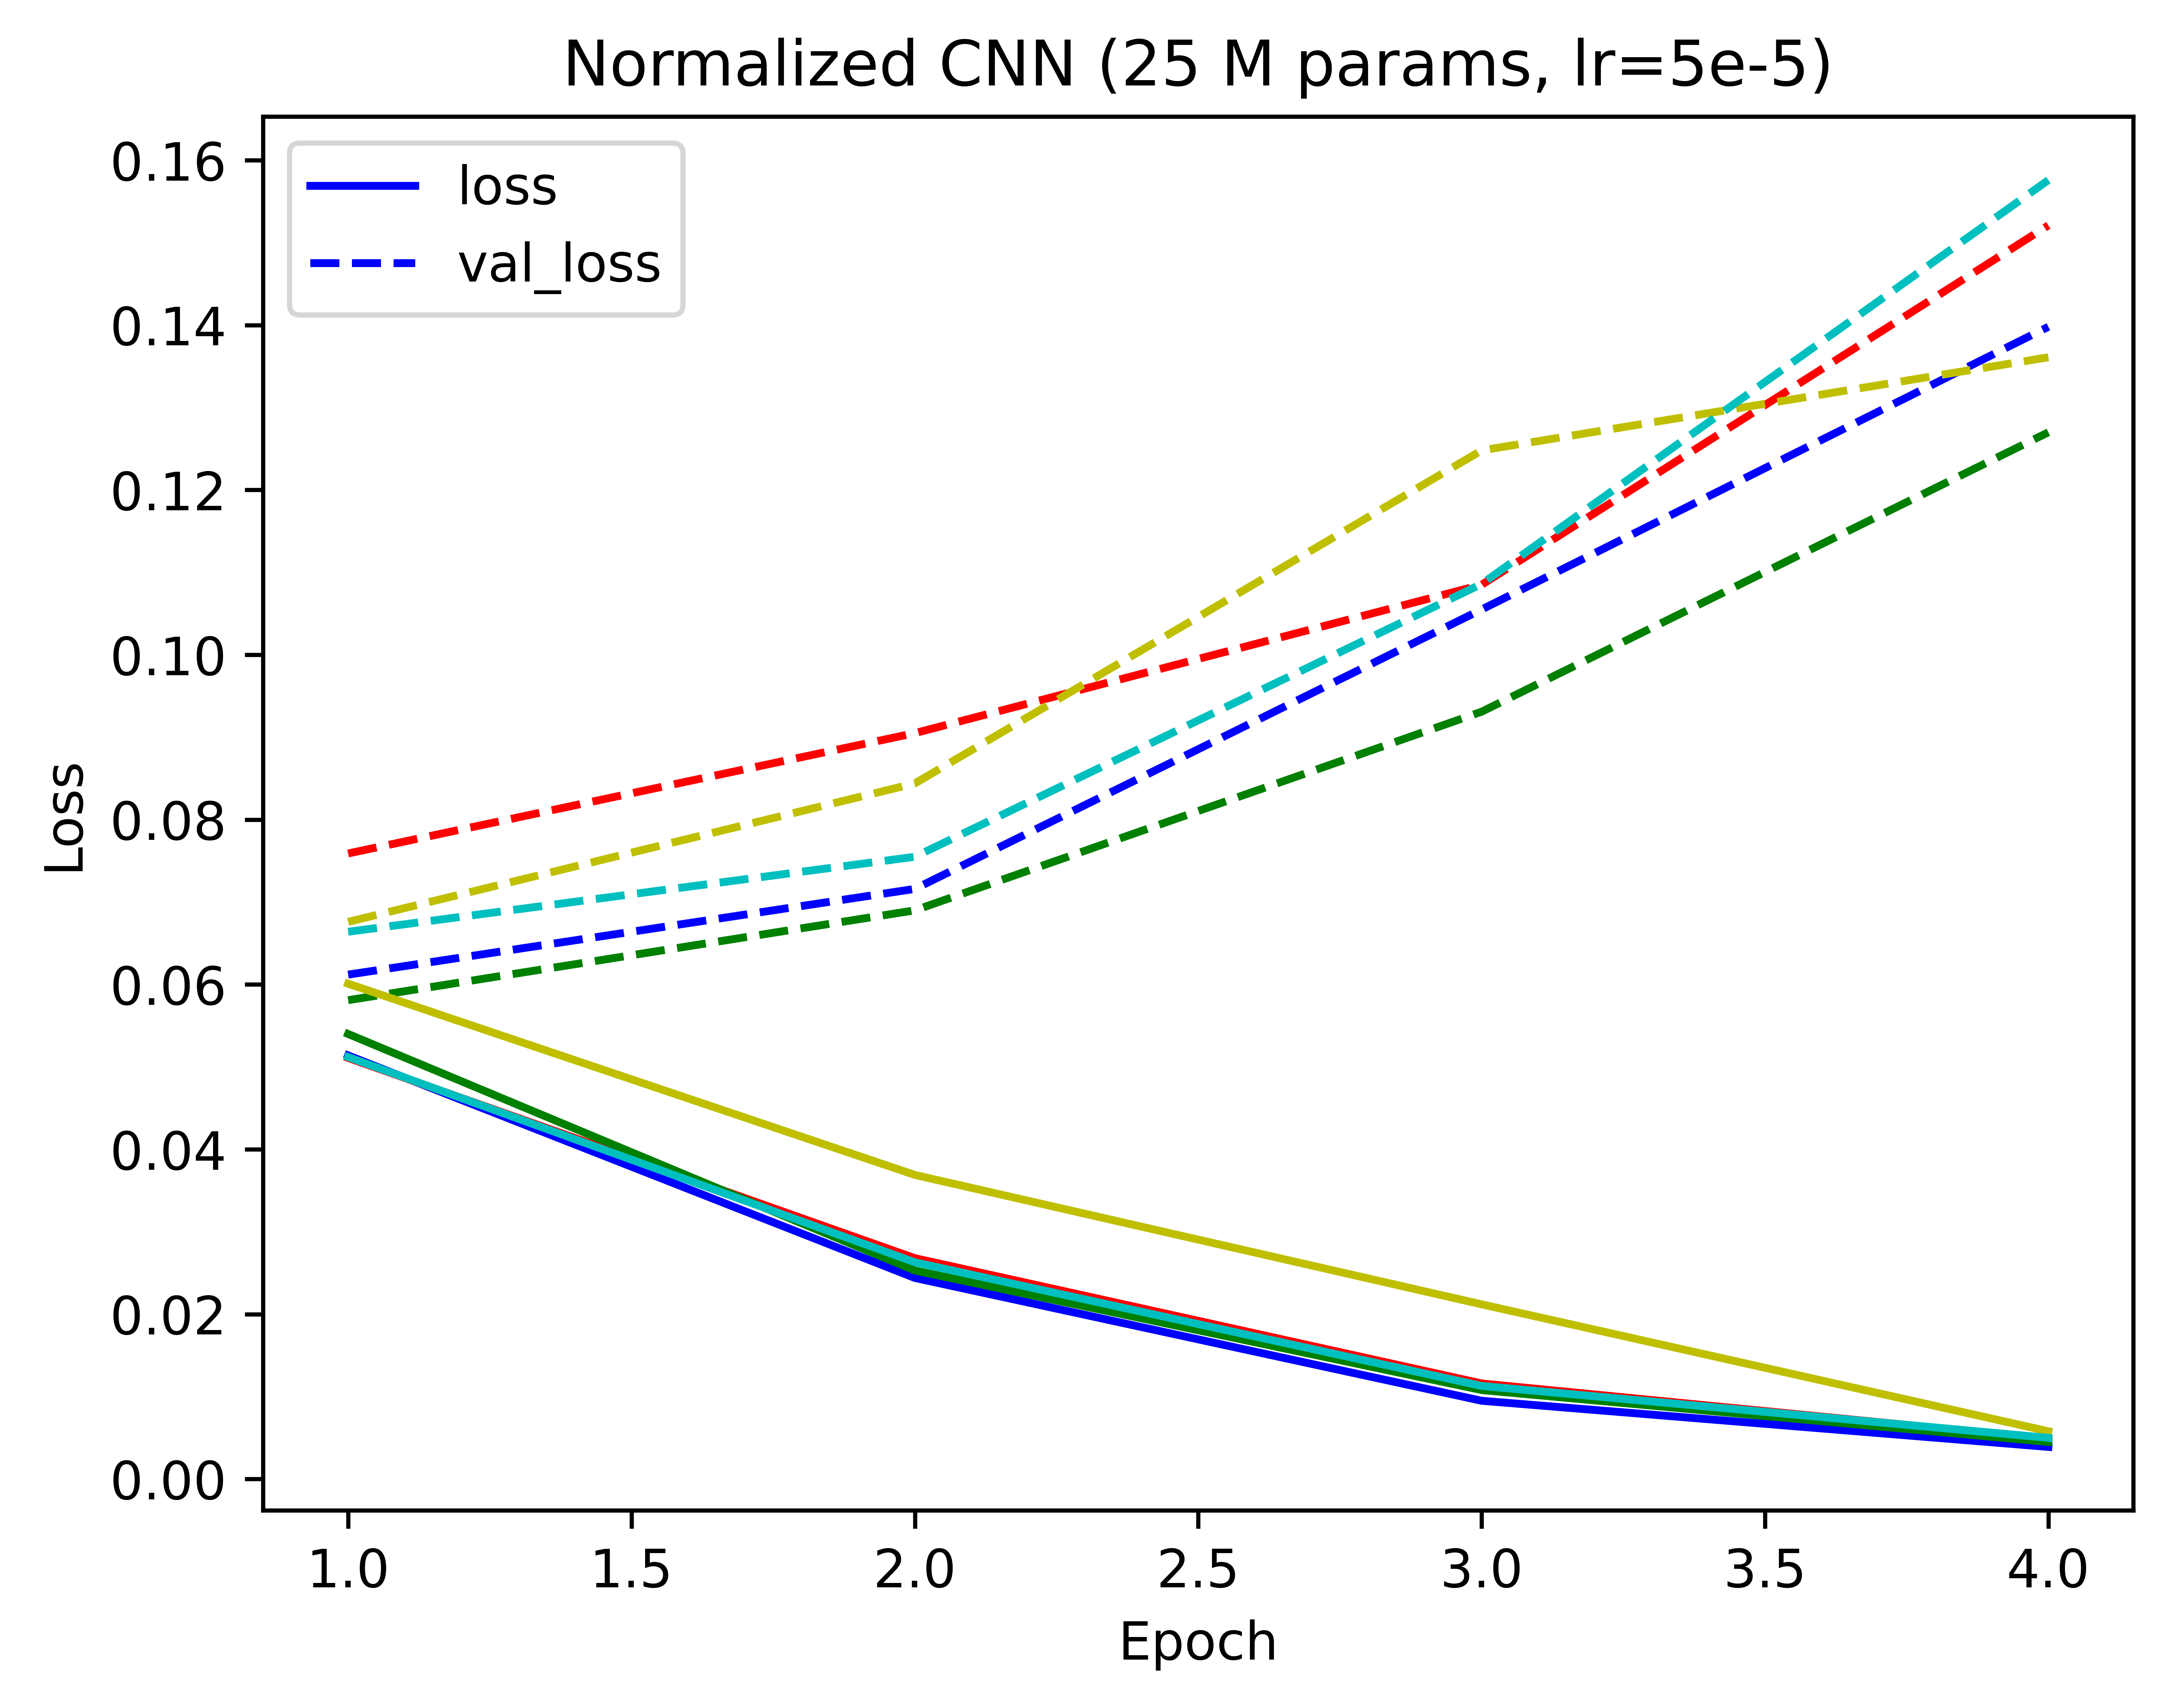
\includegraphics[width=1\linewidth]{Normalized CNN_loss.png}
\end{subfigure}
\begin{subfigure}{0.45\textwidth}
    \centering
    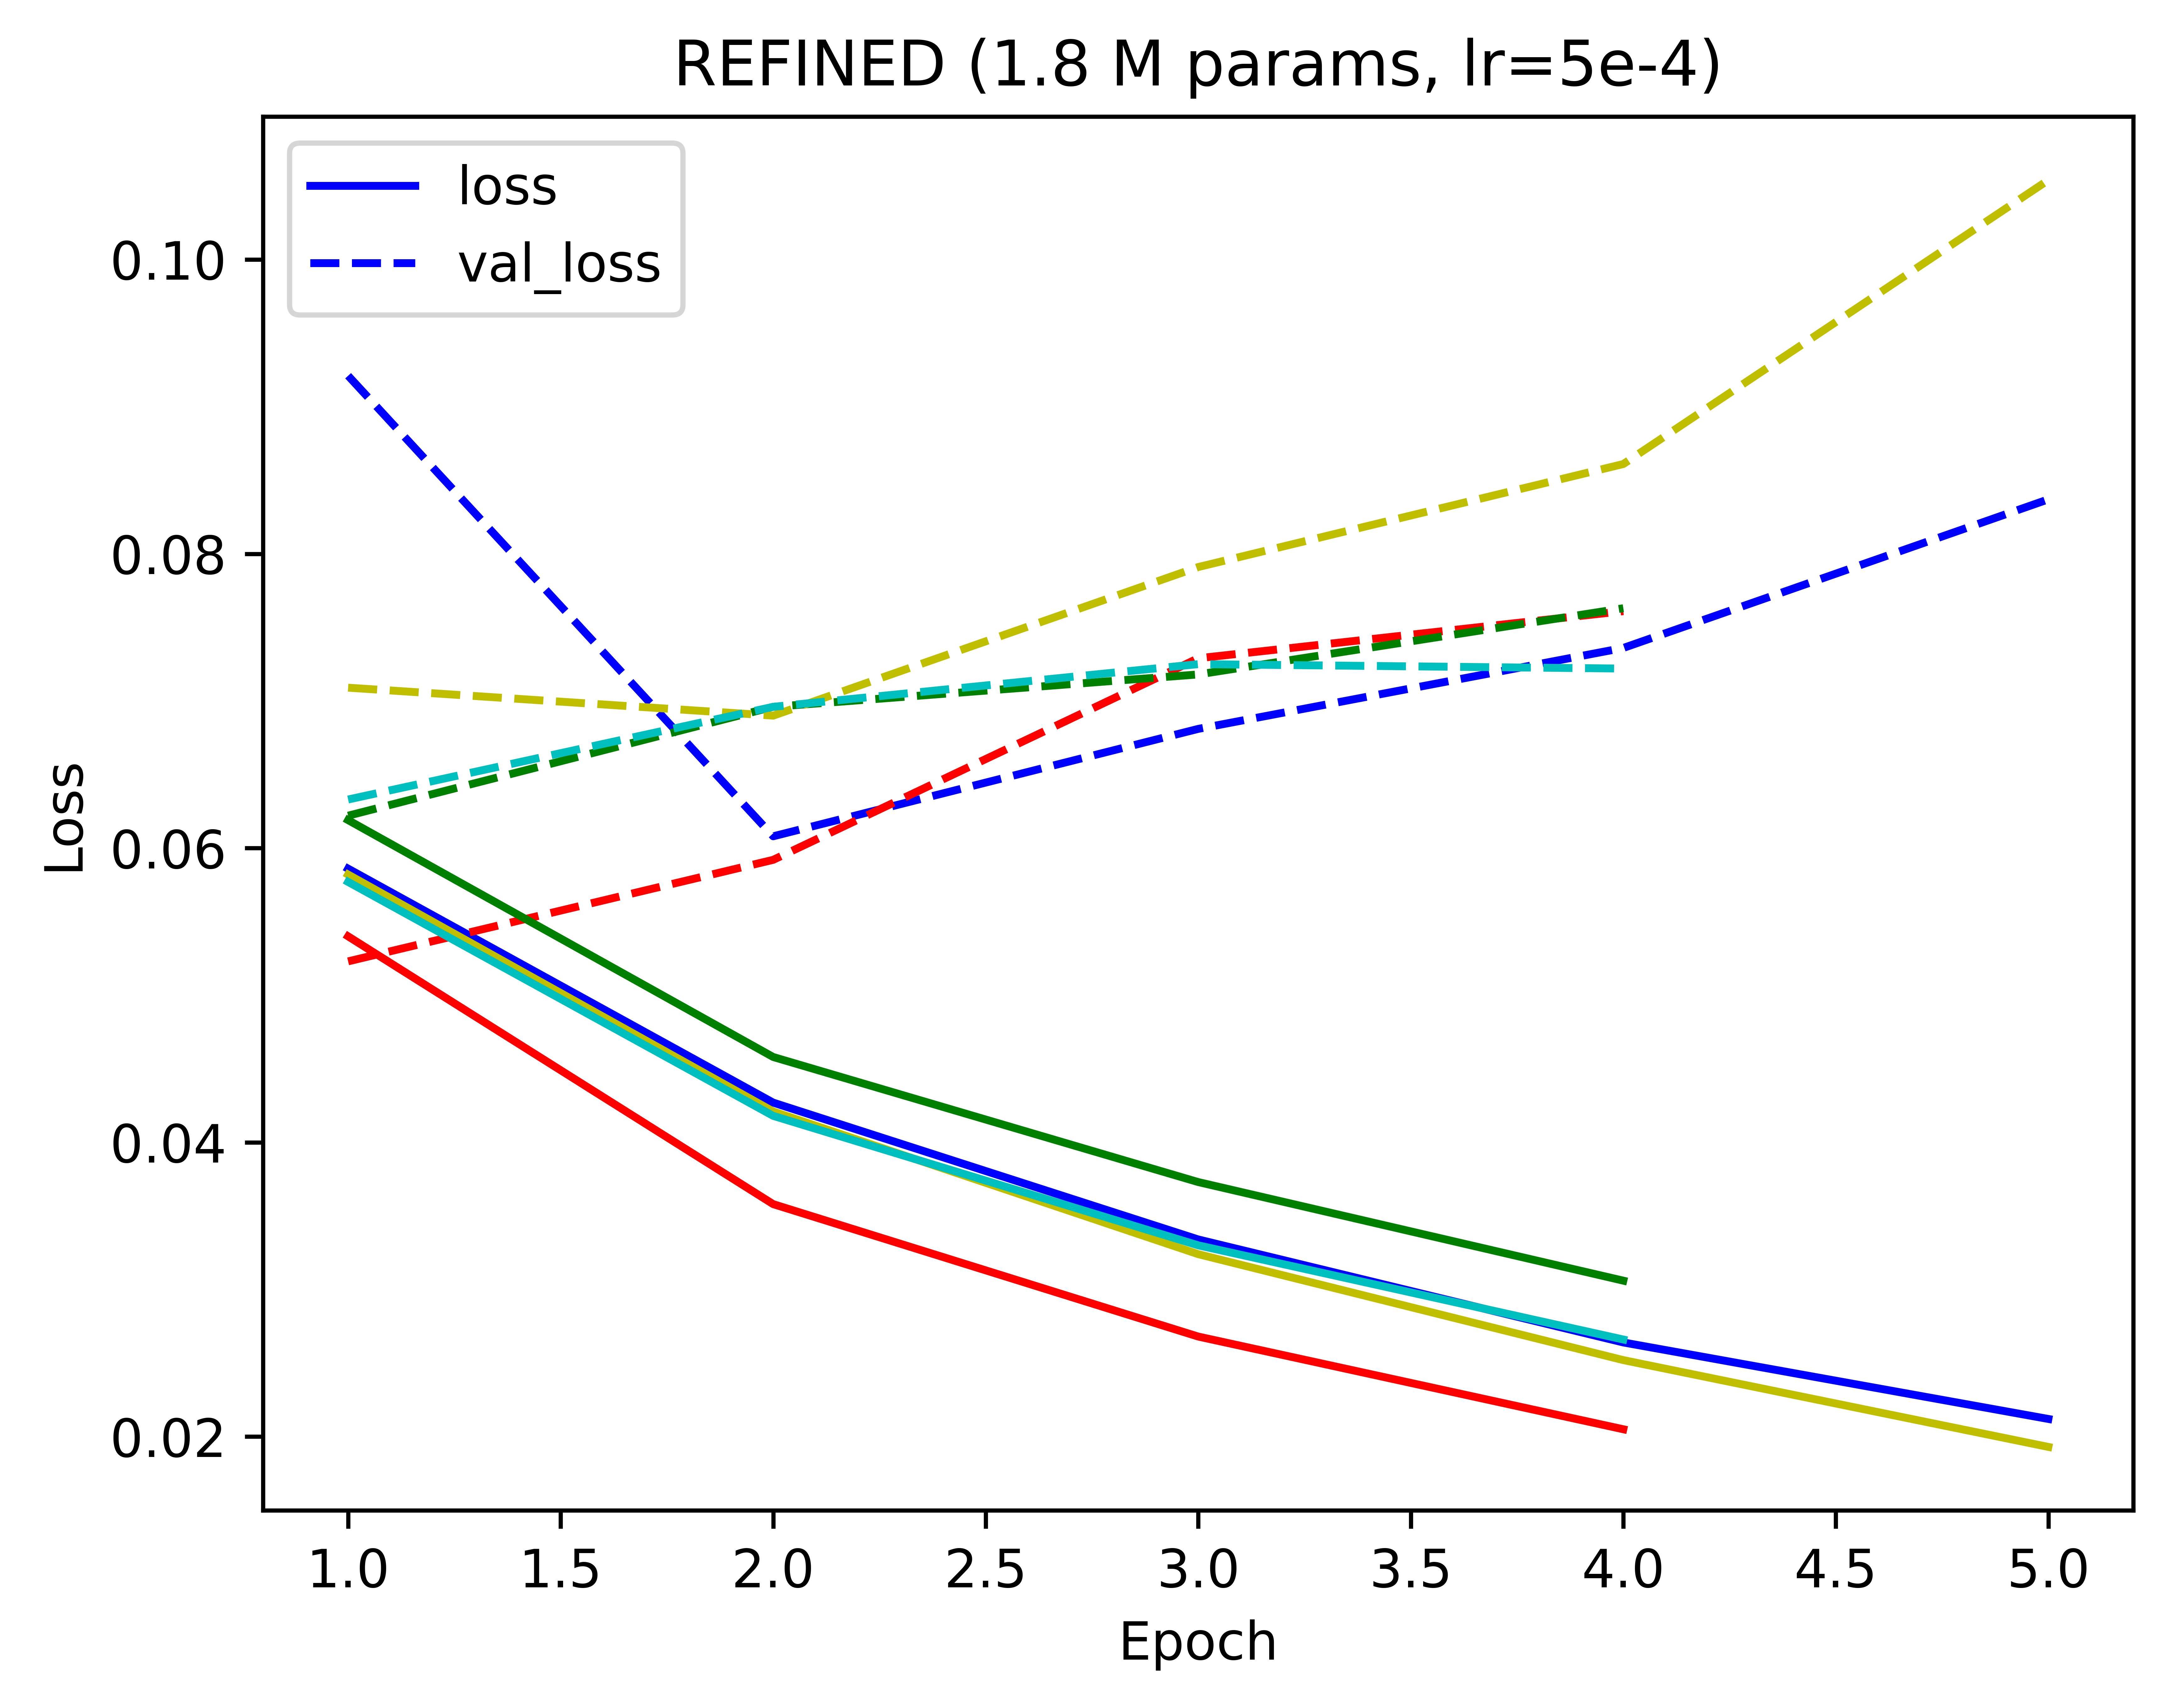
\includegraphics[width=1\linewidth]{Refined_loss.png}
\end{subfigure}%
\begin{subfigure}{0.45\textwidth}
    \centering
    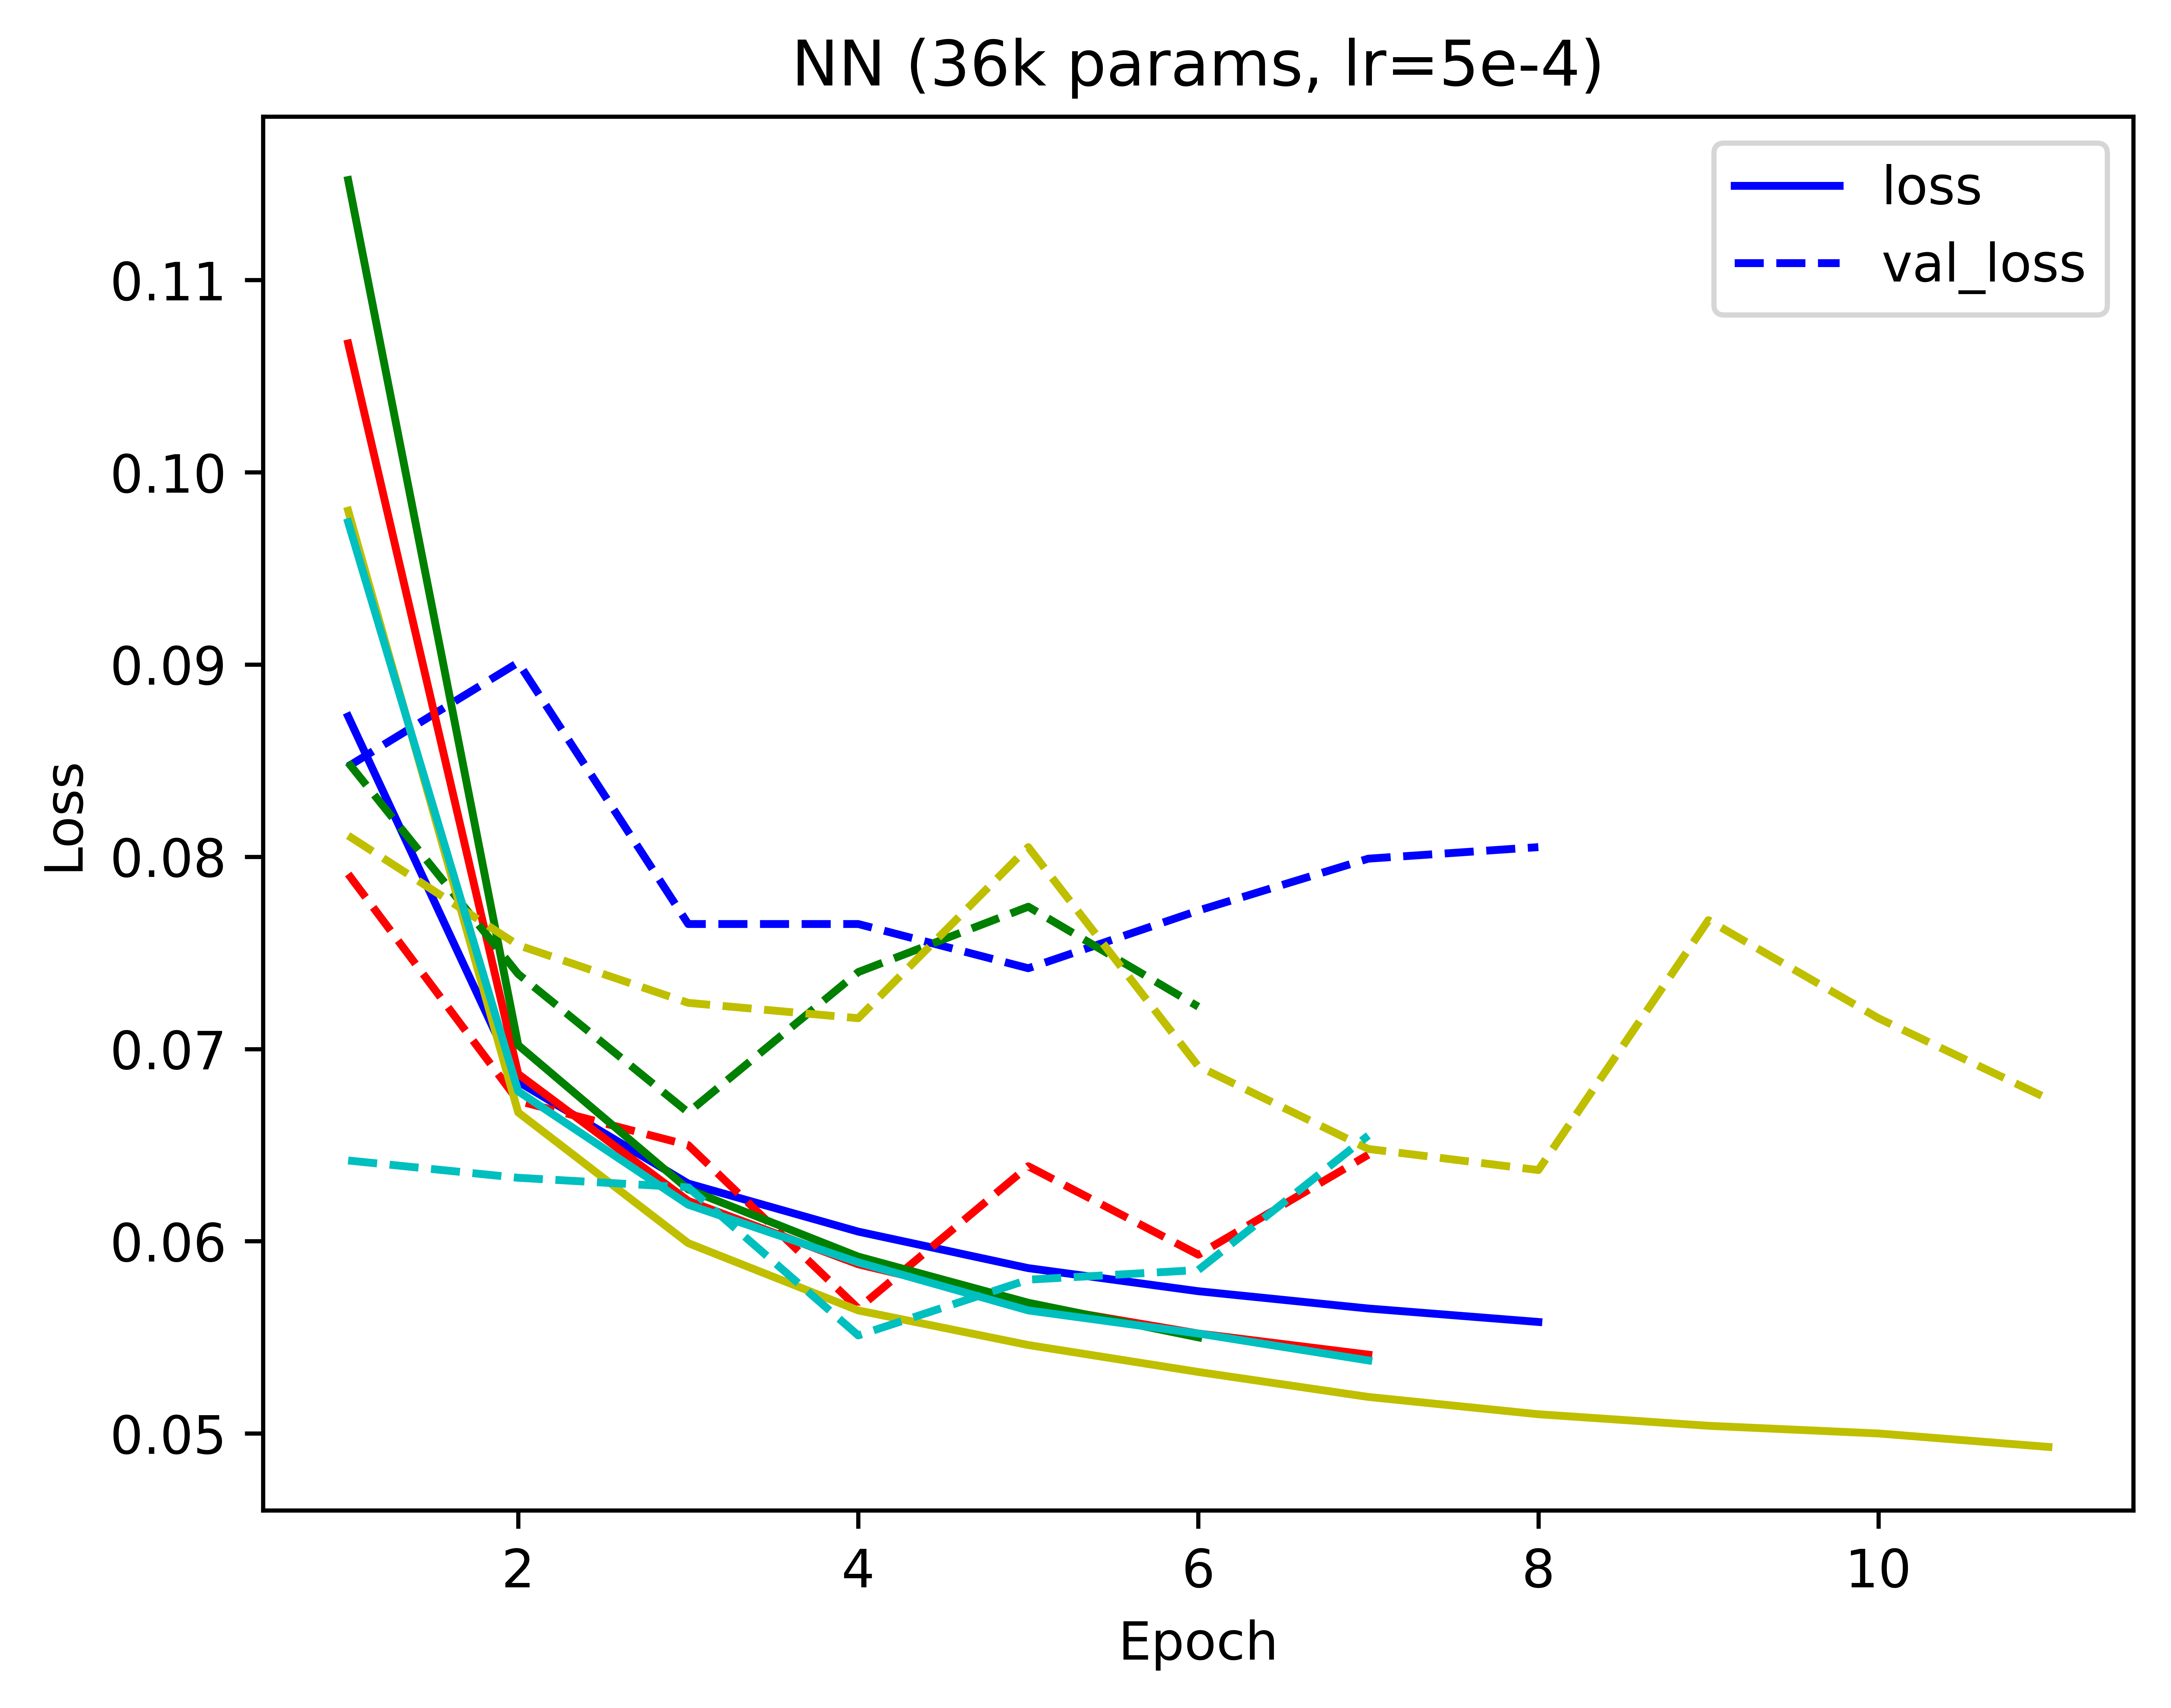
\includegraphics[width=1\linewidth]{NN_loss.png}
\end{subfigure}
\caption{Training and validation losses per epoch for each neural-based model. Early stopping with patience of 3 epochs was used for all models. Interestingly, the REFINED and Normalized CNN models achieve the best performance in the first 2 epochs in every run and then start overfitting. This is not too surprising compared to the \textit{NN} model, which is much smaller, but is surprising in the context of the \textit{Random CNN} model improving its performance for longer.}
\label{fig:enter-label}
\end{figure}
\section{REFINED progression}
With the inconclusive results of the previous experiment, I want to look more closely into how REFINED works. From the first experiment, I have saved the individual REFINED permutations. First, let's look at what they look like, and after that, let's see if there is any correlation between a CNN performance and the REFINED score on which it is based.

\subsection{REFINED visualised}

The first question asked was whether REFINED worked as intended. For this, a simple visualization, as can be seen in Figure ~\ref{fig:REFINED_visualized}, sufficed. It can be seen that the REFINED core has created some gradients in the resulting images. 

\begin{figure}
    \centering
    \includegraphics[width=1\linewidth]{positive_progression.png}
    \caption{Visualisation of different epochs of REFINED. For selected epochs, the REFINED score is shown with a visualization of the distribution of different features. To obtain the visualization, all positively labeled samples (marked as LBS) were transformed by REFINED at the given epoch (including the normalization step, which is common for all epochs), and then the mean value was plotted. It can be seen that a lot of changes are happening in the first few epochs, improving the REFINED score quickly, but only a few in the second half of the run.}
    \label{fig:REFINED_visualized}
\end{figure}

\subsection{Experiment 2: CNN performance and REFINED score}

Seeing that there is no visible improvement in the overall REFINED performance compared to the Random CNN, although the visualizations show that REFINED core works as intended, I wanted to test whether training a CNN on REFINED-transformed images produces better results than on images with randomly allocated positions. I have taken the individual epochs of REFINED and trained a CNN model on each epoch of REFINED to test this. These models were trained using the CNN hyperparameters found model in the first experiment. This should only improve the performance of models with better REFINED score.

Then, I tested whether there was any correlation between the REFINED score and CNN's performance. The obvious metric to compare is the validation loss, as it represents the training goals the best.

In ~\ref{fig:REFINED_progression}, it can be seen that there is little to no correlation between the REFINED score and the model's performance. Most of the points have a similar REFINED score, as a larger number of pixels can move in the beginning epochs of the REFINED algorithm, quickly decreasing the REFINED score. In contrast at the end only small local changes are happening, causing the clustering.

\begin{figure}
    \centering
    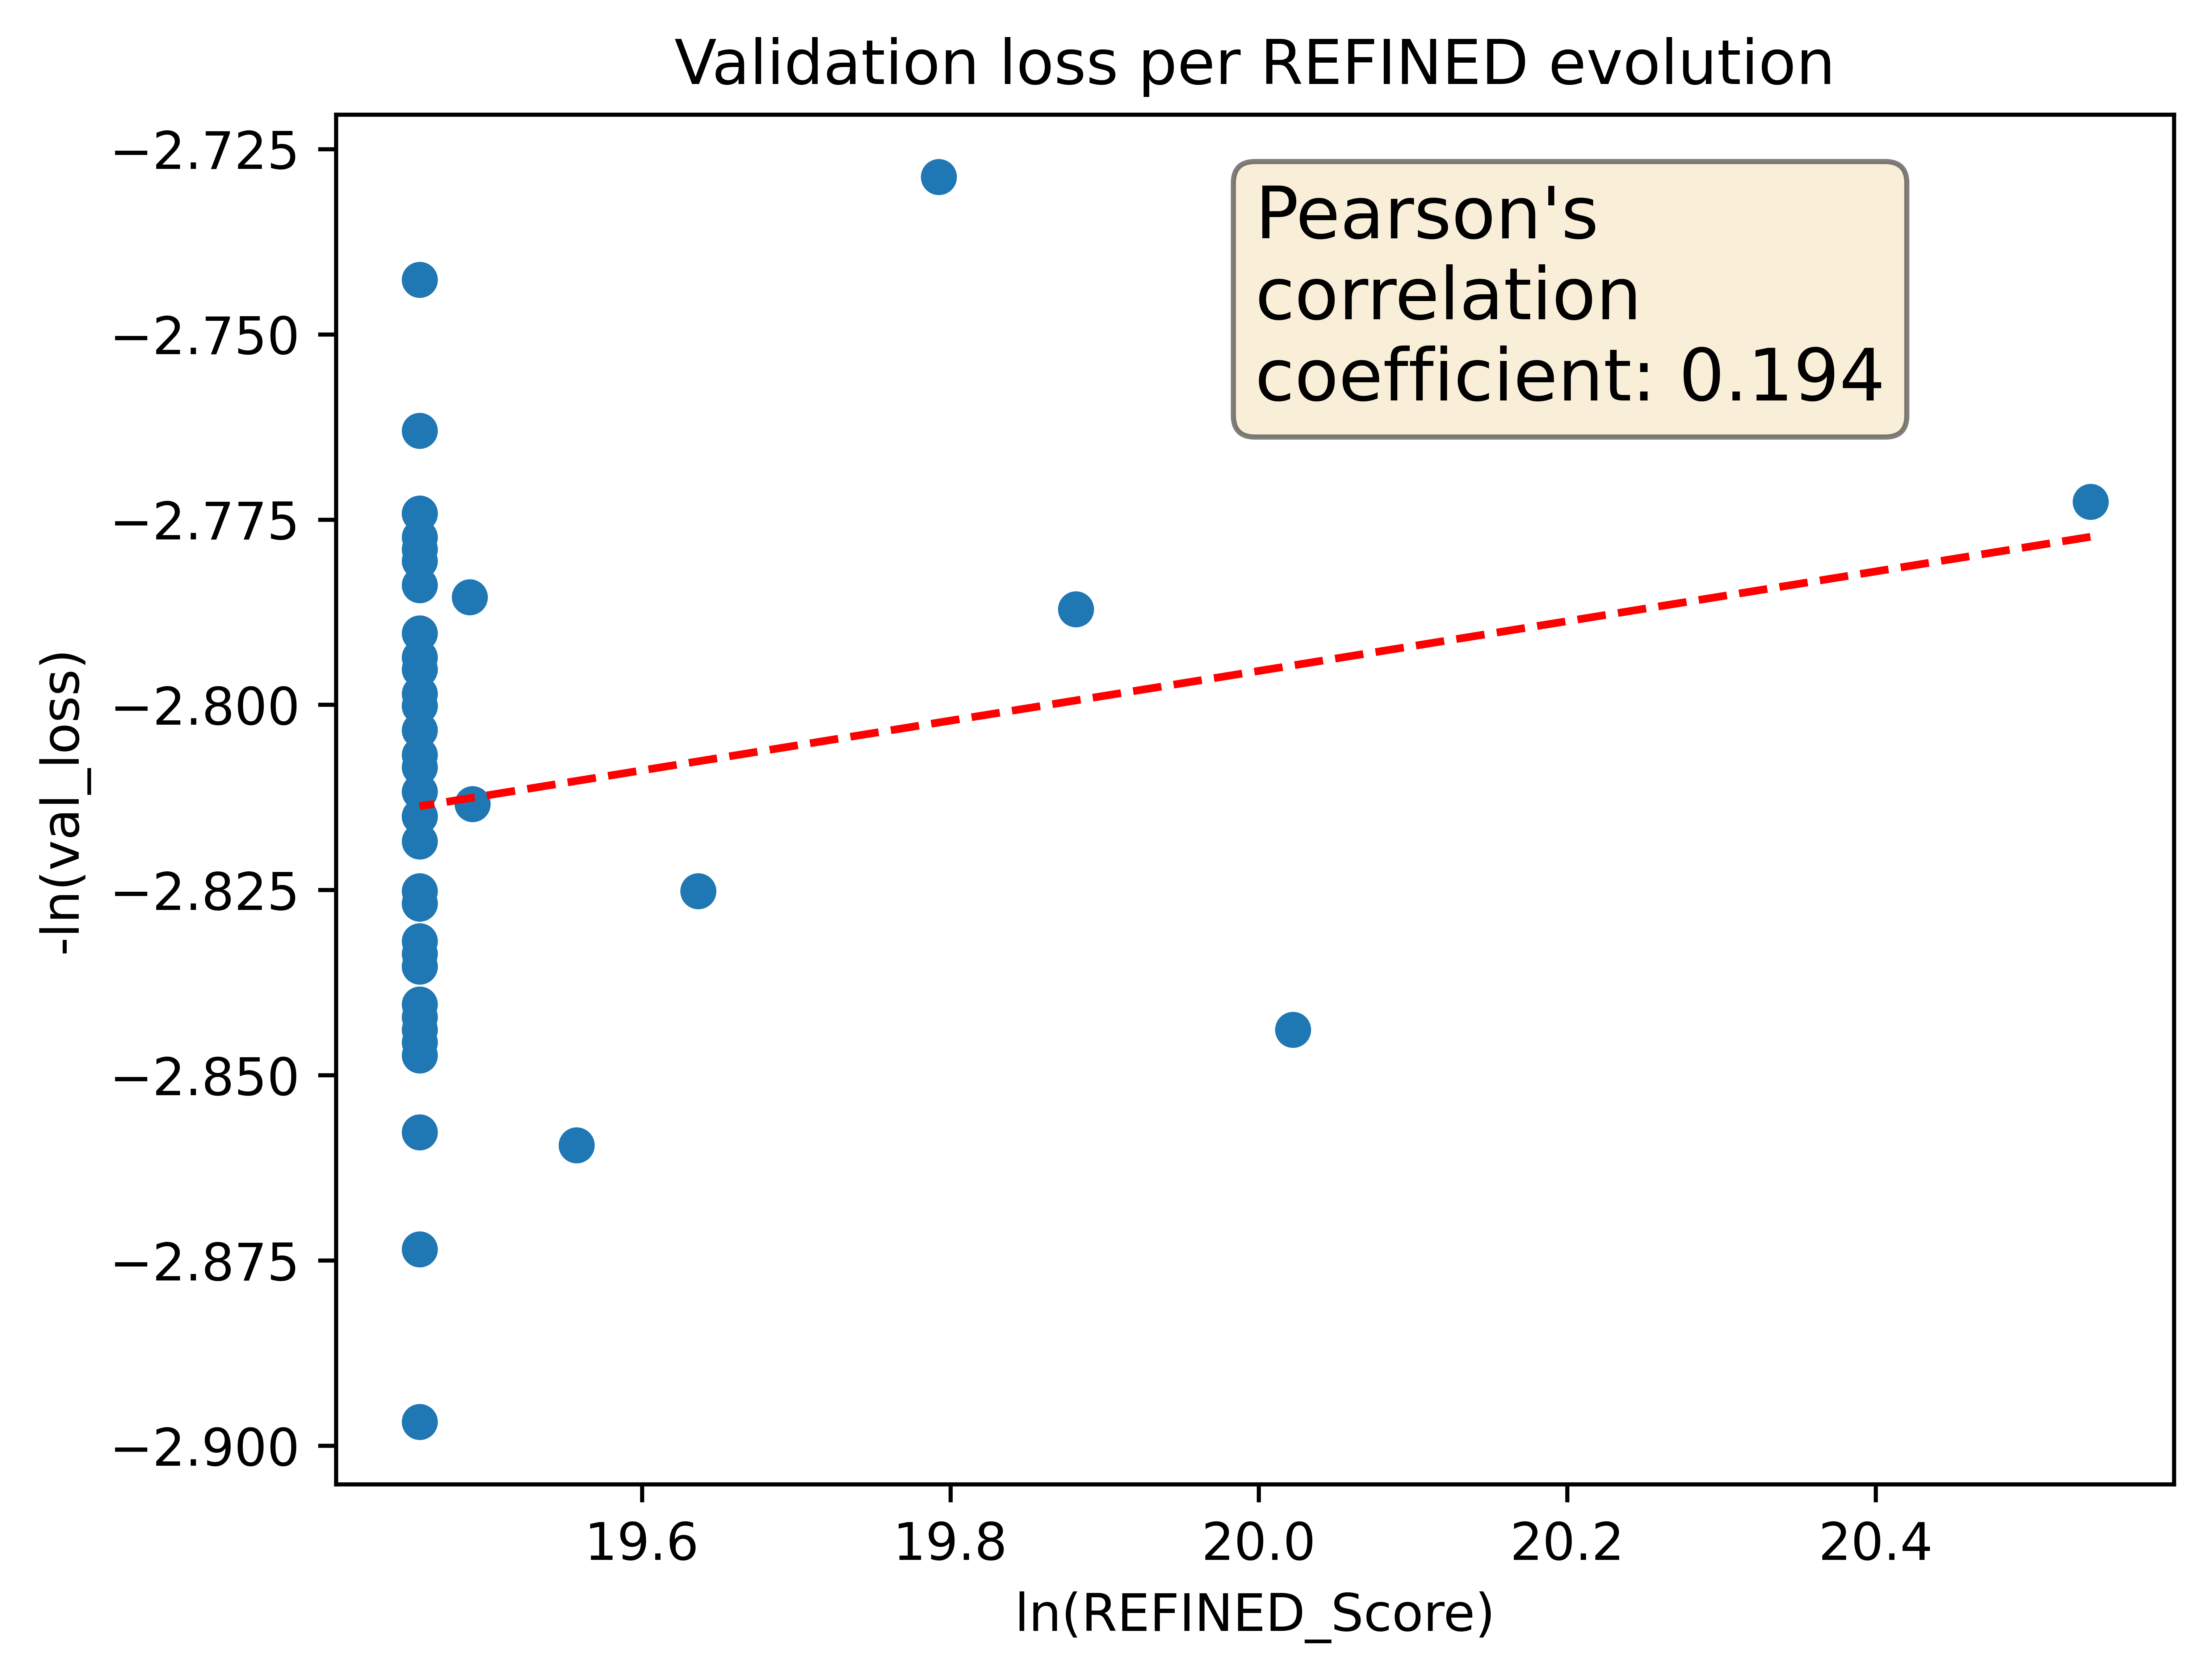
\includegraphics[width=0.75\linewidth]{progression.png}
    \caption{Best achieved CNN validation loss plotted against the REFINED score. Individual measurements are shown by the blue dots. The red line represents the least squares linear fit to the data. The Pearson's correlation coefficient between the two variables is shown in the top right corner.}
    \label{fig:REFINED_progression}
\end{figure}

